\newpage

\section{Compare the implemented procedures from questions 4 and 5 and the beta distribution generator incorporated in R in terms of their runtime (keep $n = 15,\!000$) as well as their precision (use different values of $n$).}

 We compared three methods to generate samples from the Beta distribution $\text{Be}(3, 9)$: the transformation method using uniform logarithms (Question \ref{sec:4}), the gamma ratio method (Question \ref{sec:5}), and the built-in Beta generator from the SciPy library. Runtime was measured for a fixed sample size of \(n=15,\!000\), while precision was evaluated across varying sample sizes. To ensure the stability of the test results, 200 experiments are run, and then the average results are reported.


% We compared three methods to generate samples from the Beta distribution $\text{Be}(3, 9)$:

% \begin{itemize}
%     \item Uniform Log Transformation (Question \ref{sec:4})
%     \item Gamma Ratio Method (Question \ref{sec:5})
%     \item Built-in Beta RNG from \texttt{scipy.stats.beta}
% \end{itemize}

\textbf{Runtime comparison}: The average runtimes over 200 experiments for \(n = 15,000\) samples are shown in Table~\ref{tab:runtime}.

\begin{table}[H]
\centering
\footnotesize
\noskipcaption{Average runtime in terms of 15,000 samples for Beta sampling methods.}
\label{tab:runtime}
\begin{tabular}{lccc}
\hline
Method & Transformation & Gamma ratio & Built-in Beta \\
\hline
Average Runtime (s) & 0.002252 & 0.000736 & 0.000736 \\
\hline
\end{tabular}
\end{table}

The gamma ratio and built-in methods are significantly faster than the transformation method.

\textbf{Precision comparison}: Precision is assessed using the Kolmogorov-Smirnov (K-S) statistic, quantifying the difference between the empirical and theoretical Beta distribution. Lower values indicate better precision. The average K-S statistics are computed over 200 experiments for various sample sizes.


\begin{table}[H]
\centering
\footnotesize
\noskipcaption{Average K-S statistic in terms of different sample sizes for Beta sampling methods.}
\label{tab:ks}
\begin{tabular}{lcccccc}
\hline
Sample Size (\(n\)) & 10 & 100 & 1,000 & 10,000 & 100,000 & 1,000,000 \\
\hline
Transformation & 0.2657 & 0.0853 & 0.0273 & 0.0088 & 0.0028 & 0.0009 \\
Gamma Ratio    & 0.2601 & 0.0900 & 0.0276 & 0.0088 & 0.0027 & 0.0009 \\
Built-in Beta  & 0.2575 & 0.0872 & 0.0275 & 0.0089 & 0.0028 & 0.0009 \\
\hline
\end{tabular}
\end{table}

\begin{figure}[H]
    \centering
    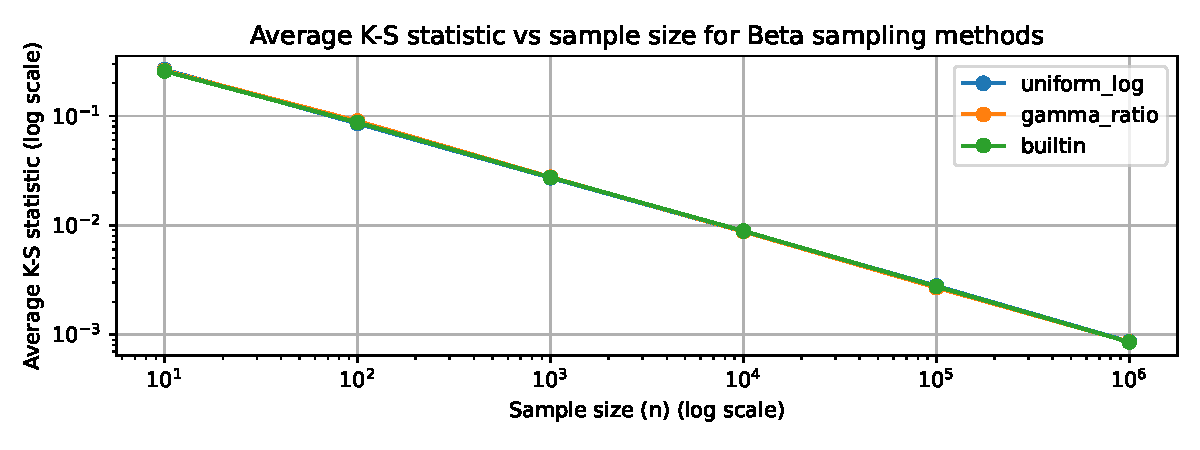
\includegraphics[width=0.7\textwidth]{resources/figures/q6-beta_sampling_methods_ks_statistic.pdf}
    \noskipcaption{Average K-S statistic in terms of different sample sizes for Beta sampling methods.}
    \label{fig:ks_stat_comparison}
\end{figure}

Table~\ref{tab:ks} and Figure~\ref{fig:ks_stat_comparison} show that all three methods yield nearly indistinguishable precision performance over a broad range of sample sizes. Differences between methods are minimal. They produce samples closely matching the Beta distribution, with K–S statistics decreasing as \(n\) grows. The K–S statistic decreases approximately linearly on the log-log scale, consistent with theoretical convergence rates.

Regarding both results, they suggest the gamma ratio and built-in methods are preferable for efficient and accurate Beta random variable generation, especially for large-scale simulations.



% In this section, we compare the performance of three different methods to generate samples from a $\text{Be}(3, 9)$ distribution:
% \begin{enumerate}
%     \item Uniform log-transformation method (Question \ref{sec:4}): based on transforming products (or negative logs) of uniform random variables when $\alpha$ and $\beta$ are integers.
%     \item Gamma ratio method (Question \ref{sec:5}): based on the property that the ratio $\frac{Y_1}{Y_1 + Y_2}$ of two Gamma variables follows a Beta distribution.
%     \item Built-in generator using \texttt{scipy.stats.beta.rvs()}, which approximates the functionality of R's \texttt{rbeta()}.
% \end{enumerate}

% \subsubsection*{Runtime comparison}

% To evaluate efficiency, we measured the runtime of each method for generating $n = 15,\!000$ samples. The recorded times (in seconds) are:

% \begin{table}[H]
%     \centering
%     \small
%     \caption{Runtime comparison for generating 15,000 samples from $\text{Be}(3, 9)$.}
%     \begin{tabular}{lc}
%         \hline
%         \textbf{Method}            & \textbf{Runtime (s)} \\
%         \hline
%         Uniform Log-transformation & 0.00251              \\
%         Gamma ratio                & 0.00099              \\
%         Built-in Beta generator    & 0.00100              \\
%         \hline
%     \end{tabular}
% \end{table}

% The Gamma ratio method is the fastest, followed closely by the built-in generator. The uniform-log method is slightly slower due to matrix-based operations.

% \subsubsection*{Precision comparison}

% To evaluate accuracy, we compared the generated samples against the true $\text{Be}(3, 9)$ distribution using three metrics:
% \begin{itemize}
%     \item Mean absolute error (MAE) between histogram and theoretical PDF
%     \item Wasserstein distance (WD) from empirical to true distribution
%     \item Kolmogorov-Smirnov statistic (KS) comparing empirical and theoretical CDFs
% \end{itemize}

% The following table summarizes the results for increasing values of $n$:

% \begin{table}[H]
%     \centering
%     \small
%     \caption{Precision comparison across methods using MAE, WD, and KS. UL = Uniform Log, G = Gamma, B = Built-in.}
%     \begin{tabular}{rccccccccc}
%         \hline
%         \textbf{$n$} & \textbf{MAE}$_{\text{UL}}$ & \textbf{MAE}$_{\text{G}}$ & \textbf{MAE}$_{\text{B}}$ & \textbf{WD}$_{\text{UL}}$ & \textbf{WD}$_{\text{G}}$ & \textbf{WD}$_{\text{B}}$ & \textbf{KS}$_{\text{UL}}$ & \textbf{KS}$_{\text{G}}$ & \textbf{KS}$_{\text{B}}$ \\
%         \hline
%         100       & 0.501 & 0.591 & 0.552 & 0.0150 & 0.0114 & 0.0153 & 0.0860 & 0.0594 & 0.0856 \\
%         1,000     & 0.188 & 0.186 & 0.176 & 0.0084 & 0.0039 & 0.0029 & 0.0416 & 0.0264 & 0.0279 \\
%         10,000    & 0.068 & 0.054 & 0.063 & 0.0016 & 0.0022 & 0.0026 & 0.0103 & 0.0091 & 0.0165 \\
%         100,000   & 0.021 & 0.017 & 0.019 & 0.0010 & 0.0008 & 0.0009 & 0.0031 & 0.0024 & 0.0034 \\
%         1,000,000 & 0.006 & 0.006 & 0.006 & 0.0006 & 0.0006 & \textbf{0.0005} & 0.0009 & 0.0009 & \textbf{0.0005} \\
%         \hline
%     \end{tabular}
% \end{table}

% % \subsubsection*{Conclusion}
% \textcolor{red}{All three methods improve in accuracy as the number of samples increases. For small sample sizes ($n = 100$), differences are more pronounced, with the Gamma ratio method generally offering better performance in terms of MAE and KS.}

% \textcolor{red}{At large sample sizes ($n \geq 100,\!000$), the built-in generator consistently performs best across most metrics. However, both the transformation and gamma ratio methods are also highly accurate and efficient.}

% \textcolor{red}{The Gamma ratio method stands out as the most efficient (fastest runtime) and provides competitive precision, making it a strong choice when both speed and general applicability are important.}












% ---

% The runtime of the different methods are displayed in the following table:

% \begin{table}[h]
%     \centering
%     \caption{Runtime for the different procedures}
%     \begin{tabular}{cc}
%         \hline
%         \textbf{Method} & \textbf{Time} \\
%         \hline
%         Transformation &  \\
%         Gamma &  \\
%         Scipy &  \\
%         \hline
%     \end{tabular}
% \end{table}

% We can see that the fastest method is the built-in method from the Python library (Scipy). This is because those kinds of functions are extremely optimized. Then the gamma method is the second fastest; it uses the gamma distribution (using the Python library and so the method is highly optimized too) to simulate random variables for a beta distribution which makes it faster than the transformation one. The slowest is the transformation method, because of the logarithm and sum operations; this requires more time because it looks up several times into an array.

% \vspace{1em}

% I decided to use the Kolmogorov-Smirnov statistic test to compare the precision of the different methods for different $n$. This test compares two samples of random variables. It can also be used to test a sample of random variables with a reference probability distribution (in our case, the beta distribution). A smaller value means that the two samples are close to each other. In other words, the smaller the value, the closer to the beta distribution the sample is. The different values obtained are displayed in the following table:

% \begin{table}[h]
% \centering
% \begin{tabular}{rccc}
% \hline
% \textbf{N} & \textbf{KS Transformation} & \textbf{KS Gamma} & \textbf{KS Scipy} \\
% \hline
% 10 &  &  &  \\
% ? &  &  &  \\
% ? &  &  &  \\
% ? &  &  &  \\
% ? &  &  &  \\
% ? &  &  &  \\
% \hline
% \end{tabular}
% \caption{KS test for different values of $n$ for the different methods}
% \end{table}

% As we can see, the higher the value of $n$, the higher the precision of the sample is (lower KS value). This is explained by the law of large numbers: larger samples are more representative of a distribution (beta distribution in our case). As I tried several runs to understand the behaviour, the results highly depend on the run (which makes sense because the samples are drawn from a probability distribution). For small values of $n$ (10 and 100), we can see that the built-in method is not the best. As $n$ increases, the KS value for the scipy method is close to the best value. However, I cannot precisely tell which method is the best in every situation. In short, the KS value of the scipy method is low and consistent, which makes it very usable.
